% Created 2022-03-09 Wed 10:36
% Intended LaTeX compiler: pdflatex
\documentclass[8pt, compress]{beamer}
\usepackage[utf8]{inputenc}
\usepackage[T1]{fontenc}
\usepackage{graphicx}
\usepackage{longtable}
\usepackage{wrapfig}
\usepackage{rotating}
\usepackage[normalem]{ulem}
\usepackage{amsmath}
\usepackage{amssymb}
\usepackage{capt-of}
\usepackage{hyperref}
\title[High-Throughput DFT Proposal]{SimTool for Rapid Simulation of Semiconductor Optical Properties of Practical Interest}
\institute[Mannodi Group and Strachan Group]{Purdue Materials Science and Engineering\\
\begin{tabular}[h]{cc}
\inst{1} Mannodi Group & \inst{2} Strachan Group\\
\end{tabular}
}
\mode<beamer>{\usetheme{Warsaw}}
\useoutertheme{miniframes}
\usetheme{default}
\author{Panayotis Manganaris\inst{1} Kat Nykiel\inst{2}}
\date{\today}
\title{Optical Properties Suite Workflow and Resulting Successes and Failures}
\hypersetup{
 pdfauthor={Panayotis Manganaris\inst{1} Kat Nykiel\inst{2}},
 pdftitle={Optical Properties Suite Workflow and Resulting Successes and Failures},
 pdfkeywords={},
 pdfsubject={},
 pdfcreator={Emacs 27.2 (Org mode 9.5)}, 
 pdflang={English}}
\begin{document}

\maketitle
\begin{frame}{Outline}
\tableofcontents
\end{frame}

\section{Input/Output}
\label{sec:org6ff28c5}
\begin{frame}[label={sec:org505ba05},fragile]{Inputs}
 \begin{columns}
\begin{column}{0.3\columnwidth}
\begin{block}{Structure Selection}
\begin{enumerate}
\item mpID, POSCARS, ciffs, etc. made into pymatgen structure
\item pmg struct is encoded as dictionary and sent to tool
\item Dictionaries can be easily checked for identity
\end{enumerate}
\end{block}
\end{column}
\begin{column}{0.7\columnwidth}
\begin{block}{Input Declaration}
\tiny
\begin{verbatim}
{'@module': 'pymatgen.core.structure',
 '@class': 'Structure',
 'charge': None,
 'lattice': {'matrix': [[1.5920500003918698, -2.7575114888687695, 0.0],
   [1.5920500003918698, 2.7575114888687695, 0.0],
   [0.0, 0.0, 5.1551]],
  'a': 3.1841000007837397,
  'b': 3.1841000007837397,
  'c': 5.1551,
  'alpha': 90.0,
  'beta': 90.0,
  'gamma': 120.00000000000001,
  'volume': 45.26276950032406},
 'sites': [{'species': [{'element': 'Zn', 'occu': 1}],
   'abc': [0.6666666666666666, 0.3333333333333333, 0.5],
   'xyz': [1.5920500003918696, -0.9191704962895898, 2.57755],
   'label': 'Zn',
   'properties': {}},
  {'species': [{'element': 'Zn', 'occu': 1}],
   'abc': [0.3333333333333333, 0.6666666666666666, 0.0],
   'xyz': [1.5920500003918696, 0.9191704962895898, 0.0],
   'label': 'Zn',
   'properties': {}},
  {'species': [{'element': 'O', 'occu': 1}],
   'abc': [0.6666666666666666, 0.3333333333333333, 0.8803099999999999],
   'xyz': [1.5920500003918696, -0.9191704962895898, 4.538086080999999],
   'label': 'O',
   'properties': {}},
  {'species': [{'element': 'O', 'occu': 1}],
   'abc': [0.3333333333333333, 0.6666666666666666, 0.3803099999999999],
   'xyz': [1.5920500003918696, 0.9191704962895898, 1.9605360809999997],
   'label': 'O',
   'properties': {}}]}
\end{verbatim}
\end{block}
\end{column}
\end{columns}
\end{frame}
\begin{frame}[allowframebreaks]{Outputs}
\begin{block}{structures/chemistries returned for future query}
Outputs can be queried by key and filtered by conditional matching on values
\begin{itemize}
\item Formula
\item mpID
\item spacegroup
\end{itemize}
\end{block}
\begin{block}{Electronic properties returned for analysis}
\begin{itemize}
\item[{$\square$}] scalers
\begin{itemize}
\item[{$\square$}] bandgap
\item[{$\square$}] fermi energy
\item[{$\square$}] charge densities
\item[{$\square$}] raman/IR cutoff
\item[{$\square$}] UV cutoff
\end{itemize}
\item[{$\boxminus$}] spectra
\begin{itemize}
\item[{$\boxtimes$}] raman/IR
\item[{$\square$}] eDoS + Band-structure
\item[{$\square$}] phonon dispersion
\item[{$\square$}] SLME (these might be relegated to post processing)
\item[{$\square$}] PV FOM
\end{itemize}
\end{itemize}
\end{block}
\end{frame}
\section{Results}
\label{sec:orgeebf0b9}
\begin{frame}[allowframebreaks]{Kat's Troubleshooting in ZnO (mpid = 2133)}
Detailed breakdown of simulation shortcomings
\begin{itemize}
\item Testing workflow for ZnO (mpid = 2133)
\item outputs are \alert{extremely} sensitive to input choices
\item trying other structures would be useful as well
\end{itemize}
\begin{block}{ecutwfc = 40 Ry, 4 nodes}
\begin{center}
\begin{tabular}{rl}
KPOINTS & output\\
\hline
3 & Y\\
6 & N (vc-relax fails)\\
9 & N (vc-relax fails)\\
\end{tabular}
\end{center}
\end{block}
\begin{block}{ecutwfc = 40 Ry, 8 nodes}
\begin{center}
\begin{tabular}{rl}
KPOINTS & output\\
\hline
3 & Y\\
6 & N (vc-relax fails)\\
9 & N (vc-relax fails)\\
\end{tabular}
\end{center}
\end{block}
\begin{block}{ecutwfc = 50 Ry, 1 node}
\begin{center}
\begin{tabular}{rl}
KPOINTS & output\\
\hline
3 & Y\\
6 & N (smearing is needed)\\
9 & N (walltime reached)\\
12 & N (walltime reached)\\
15 & N (walltime reached)\\
\end{tabular}
\end{center}
\end{block}
\begin{block}{ecutwfc = 50 Ry, 4 nodes}
\begin{center}
\begin{tabular}{rl}
KPOINTS & output\\
\hline
3 & Y\\
6 & N (vc-relax fails)\\
9 & Y\\
12 & N (walltime reached)\\
15 & N (walltime reached)\\
\end{tabular}
\end{center}
\end{block}
\begin{block}{ecutwfc = 60 Ry, 4 nodes}
Is this too high? \textasciitilde{}800 eV, but 'recommended'\ldots{}
\begin{center}
\begin{tabular}{rl}
KPOINTS & output\\
\hline
3 & N (vc-relax fails)\\
6 & N (vc-relax fails)\\
9 & N (vc-relax fails)\\
\end{tabular}
\end{center}
\end{block}
\end{frame}
\begin{frame}[allowframebreaks]{Kat's Troubleshooting in SiC (mpid = 1002206)}
\begin{block}{ecutwfc = 40 Ry, 4 nodes}
\begin{center}
\begin{tabular}{rl}
KPOINTS & output\\
\hline
3 & Y\\
6 & N (vc-relax fails)\\
9 & N (vc-relax fails)\\
\end{tabular}
\end{center}
\end{block}
\end{frame}
\begin{frame}[allowframebreaks]{Convergence Plots}
\begin{block}{Convergence for 3 Kpoints}
\begin{figure}[htbp]
\centering
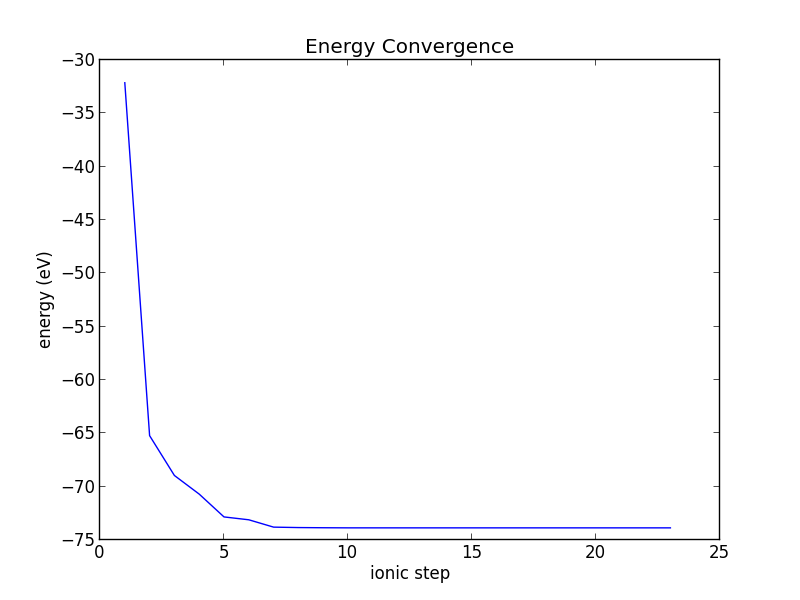
\includegraphics[width=180]{/home/panos/src/opt_prop_suite/convergence_plots/SiC_E40_K3.png}
\caption{\label{fig:Sice40k3} convergence trend at ecutwfc = 40 Ry}
\end{figure}
\end{block}
\begin{block}{9 Kpoints fails to make any ionic iteration in vcrelax}
\begin{figure}[htbp]
\centering
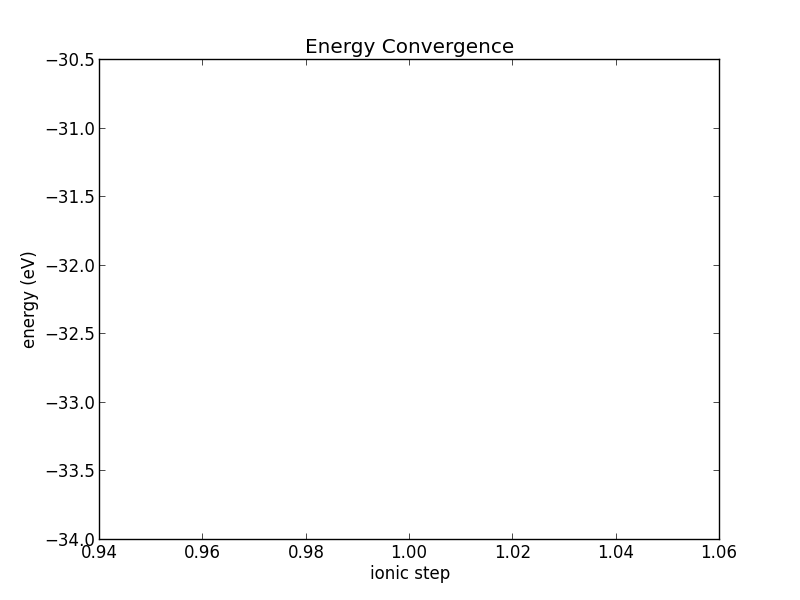
\includegraphics[width=180]{/home/panos/src/opt_prop_suite/convergence_plots/SiC_E40_K9.png}
\caption{\label{fig:Sice40k9} unfortunately blank at ecutwfc = 40 Ry}
\end{figure}
\end{block}
\end{frame}
\begin{frame}[label={sec:org5a679bd}]{Discussion}
\begin{itemize}
\item each (successful) simulation takes up 1-2 GB in storage?
\item why are they failing to converge?
\begin{itemize}
\item vcrelax final scf calculation fails to converge, even after 1000 electronic steps
\begin{itemize}
\item only one ionic step
\end{itemize}
\item "The maximum number of steps has been reached."
\end{itemize}
\item cell shape changes drastically (due to no symmetry?)
\begin{itemize}
\item we've not yet attempted replacing vc relax with atomic relax in the pipeline
\end{itemize}
\end{itemize}
\end{frame}
\section{Logistics}
\label{sec:org01d6653}
\begin{frame}[label={sec:orge7dbfa6}]{Run DB}
\begin{block}{Run Storage and Parallelization Technical Points}
\begin{itemize}
\item Currently very limited by storage space in nanoHUB
\item Each (successful) simulation takes up 1-2 GB in storage?
\item it may be desirable to reimplement the simtool via a pegasus workflow
\begin{itemize}
\item may enable improved job parallelization
\item enables more detailed data management
\end{itemize}
\end{itemize}
\end{block}
\end{frame}
\end{document}